%%%%%%%%%%%%%%%%%%%%%%%%%%%%%%%%%%%%%%%%%%%%%%%%%%%%%%%%%%%%%%%%%%%%%%%%%%%%%%%%%%%%%%%%%%

\UC{Visualizzazione ordini effettuati}
\label{visualizzazione-ordini-effettuati}

L'acquirente può visualizzare l'elenco degli ordini effettuati sulla piattaforma.
\begin{itemize}
    \item \textbf{Attori primari:} acquirente;
    \item \textbf{Precondizione:} l'acquirente si trova in una qualsiasi altra schermata e seleziona la funzionalità per accedere all'elenco degli ordini effettuati sulla piattaforma;
    \item \textbf{Postcondizione:} l'acquirente visualizza l'elenco degli ordini effettuati sulla piattaforma in ordine cronologico decrescente;
    \item \textbf{Scenario principale:} l'acquirente si trova in una qualsiasi altra schermata e seleziona la funzionalità per accedere all'elenco degli ordini effettuati sulla piattaforma. In seguito visualizzerà l'elenco degli ordini effettuati sulla piattaforma, dove è indicato per ogni ordine:
    \begin{itemize}
        \item Il codice dell'ordine;
        \item Lo stato dell'ordine;
        \item Il prezzo totale che è stato pagato;
        \item L'indirizzo a cui è stato consegnato o verrà consegnato;
        \item Una lista di tutti i prodotti acquistati in quell'ordine, dove per ogni prodotto verrà visualizzato:
        \begin{itemize}
            \item Nome del prodotto;
            \item Quantità acquistata;
            \item Prezzo totale del prodotto a cui è stato acquistato.
        \end{itemize}
    \end{itemize}
    \item \textbf{Scenari alternativi:} 
    \begin{enumerate}[label=\lett]
        \item L'acquirente non ha ancora effettuato ordini, viene visualizzato il messaggio "Nessun ordine effettuato" e sarà data la possibilità all'acquirente di tornare alla schermata principale per iniziare gli acquisti.
    \end{enumerate}
\end{itemize}

%%%%%%%%%%%%%%%%%%%%%%%%%%%%%%%%%%%%%%%%%%%%%%%%%%%%%%%%%%%%%%%%%%%%%%%%%%%%%%%%%%%%%%%%%%

\UC{Ricerca per codice di un ordine effettuato}
\label{ricerca-codice-ordine-acquirente}

L'acquirente può cercare un ordine sapendo il suo codice identificativo.
\begin{itemize}
    \item \textbf{Attori primari:} acquirente;
    \item \textbf{Precondizione:} l'acquirente si trova nella schermata di visualizzazione degli ordini effettuati e ha selezionato l'azione di ricerca per codice;
    \item \textbf{Postcondizione:} l'acquirente visualizzerà l'ordine con il codice inserito;
    \item \textbf{Scenario principale:} l'acquirente si trova nella schermata di visualizzazione degli ordini effettuati e vuole visualizzare un ordine con uno specifico codice. Per farlo dovrà selezionare la funzionalità di ricerca per codice, inserirlo e, in seguito, verrà visualizzato l'ordine interessato.
    \item \textbf{Scenari alternativi:}
    \begin{enumerate}[label=\lett]
    	\item L'acquirente ha svolto una ricerca che non ha trovato coincidenze con nessun ordine effettuato. In questo caso la schermata di visualizzazione degli ordini effettuati viene aggiornata mostrando il messaggio nessun ordine trovato.
    \end{enumerate}
    \item \textbf{Estensioni:}
    \begin{enumerate}[label=\lett]
        \item L'acquirente inserisce un codice che non rispetta il formato standard uuid v4. In questo caso:
        \begin{itemize}
            \item (UC\ref{estensione:codice-ordine-non-valido}) - Verrà visualizzato il messaggio d'errore codice dell'ordine non valido;
            \item Non verrà eseguita la ricerca.
        \end{itemize}
    \end{enumerate}
\end{itemize}

%%%%%%%%%%%%%%%%%%%%%%%%%%%%%%%%%%%%%%%%%%%%%%%%%%%%%%%%%%%%%%%%%%%%%%%%%%%%%%%%%%%%%%%%%%

\UC{Filtro temporale per gli ordini effettuati}
\label{filtro-temporale-ordini-acquirente}

\begin{figure}[H]
    \centering
    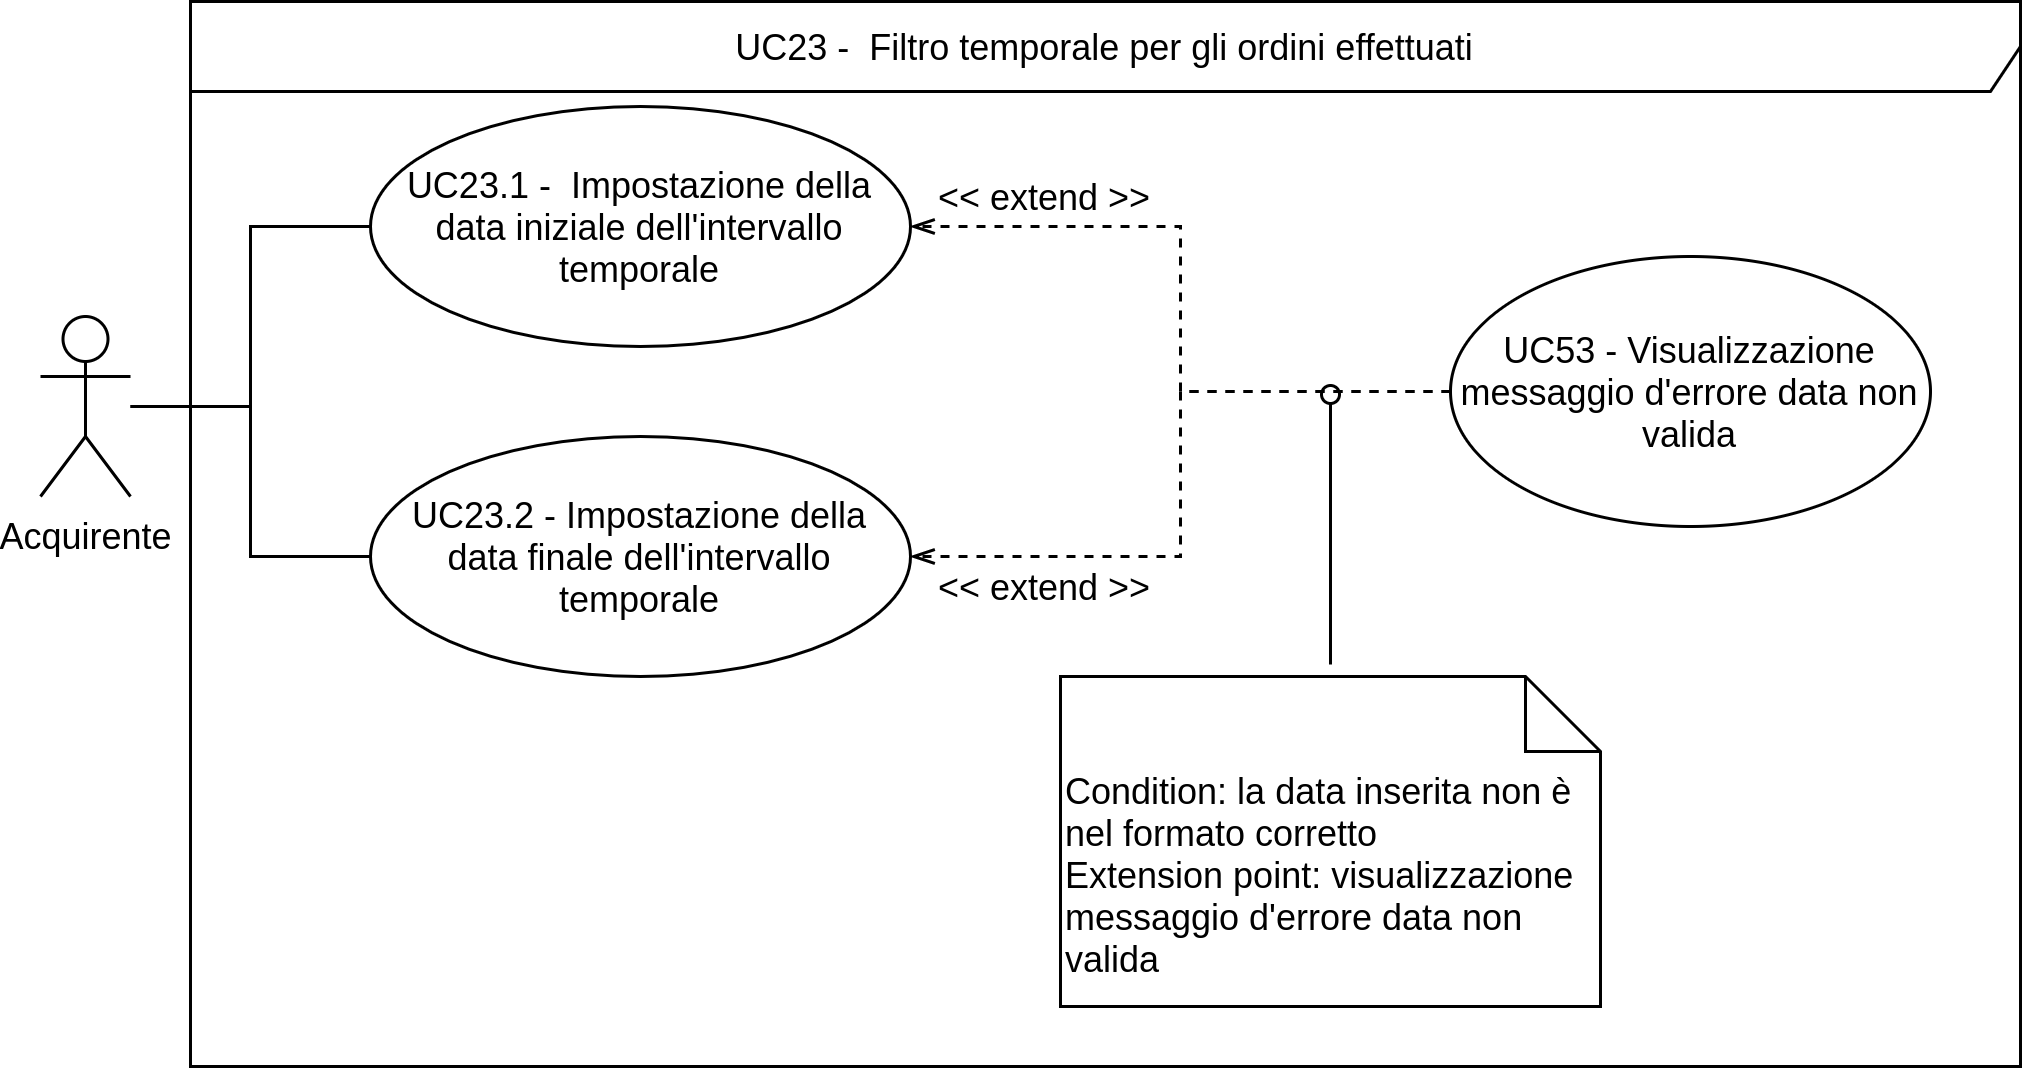
\includegraphics[scale=0.5]{Immagini/DiagrammiUC/Acquirente/FiltroTemporaleAcquirente.png}
    \caption{Diagramma di \actualUC: Filtro temporale per gli ordini effettuati dell'acquirente}
    \label{fig:filtro-temporale-ordini-acquirente}
\end{figure}

L'acquirente filtra temporalmente l'elenco degli ordini effettuati sulla piattaforma.
\begin{itemize}
    \item \textbf{Attori primari:} acquirente;
    \item \textbf{Precondizione:} l'acquirente si trova nella schermata di visualizzazione degli ordini effettuati;
    \item \textbf{Postcondizione:} l'acquirente visualizzerà tutti gli ordini che sono stati fatti tra la data di inizio e quella di fine impostate;
    \item \textbf{Scenario principale:} l'acquirente si trova nella schermata di visualizzazione degli ordini effettuati e vuole filtrare gli ordini effettuati durante un certo intervallo temporale. Per farlo dovrà:
    \begin{itemize}
        \item (UC\ref{filtro-temporale-ordini-acquirente.data-iniziale}) - Impostare la data iniziale dell'intervallo temporale;
        \item (UC\ref{filtro-temporale-ordini-acquirente.data-finale}) - Impostare la data finale dell'intervallo temporale.
    \end{itemize}
	\item \textbf{Scenari alternativi:}
	\begin{enumerate}[label=\lett]
		\item Se l'acquirente non imposta il seguente filtro, allora verranno visualizzati tutti gli ordini dal più al meno recente.
		\item L'acquirente ha impostato il filtro in modo tale che la ricerca non dia alcun risultato. In questo caso la schermata di visualizzazione degli ordini effettuati viene aggiornata mostrando il messaggio nessun ordine trovato.
	\end{enumerate}
    \item \textbf{Estensioni:}
    \begin{enumerate}[label=\lett]
        \item L'acquirente inserisce una data iniziale maggiore di quella finale. In questo caso:
        \begin{itemize}
            \item (UC\ref{estensione:data-iniziale-maggiore-data-finale}) - Verrà visualizzato il messaggio d'errore data iniziale maggiore di quella finale;
            \item Non verrà eseguita la ricerca.
        \end{itemize}
    \end{enumerate}
\end{itemize}

\subUC{Impostazione della data iniziale dell'intervallo temporale}
\label{filtro-temporale-ordini-acquirente.data-iniziale}

L'acquirente imposta la data iniziale dell'intervallo per il quale filtrare l'elenco degli ordini effettuati sulla piattaforma.
\begin{itemize}
    \item \textbf{Attori primari:} acquirente;
    \item \textbf{Precondizione:} l'acquirente si trova nella schermata di visualizzazione degli ordini effettuati;
    \item \textbf{Postcondizione:} l'acquirente ha impostato la data iniziale dell'intervallo per la quale filtrare l'elenco degli ordini effettuati sulla piattaforma;
    \item \textbf{Scenario principale:} l'acquirente si trova nella schermata di visualizzazione degli ordini effettuati e inserisce una data valida e minore o uguale a quella finale, come data iniziale dell'intervallo per la quale filtrare l'elenco degli ordini effettuati;
    \item \textbf{Estensioni:}
    \begin{enumerate}[label=\lett]
        \item L'acquirente inserisce una data iniziale non nel formato corretto. In questo caso:
        \begin{itemize}
            \item (UC\ref{estensione:data-non-valida}) - Verrà visualizzato il messaggio d'errore data non valida;
            \item Non verrà eseguita la ricerca.
        \end{itemize} 
    \end{enumerate}
\end{itemize}

\subUC{Impostazione della data finale dell'intervallo temporale}
\label{filtro-temporale-ordini-acquirente.data-finale}

L'acquirente imposta la data finale dell'intervallo per il quale filtrare l'elenco degli ordini effettuati sulla piattaforma.
\begin{itemize}
    \item \textbf{Attori primari:} acquirente;
    \item \textbf{Precondizione:} l'acquirente si trova nella schermata di visualizzazione degli ordini effettuati;
    \item \textbf{Postcondizione:} l'acquirente ha impostato la data finale dell'intervallo per la quale filtrare l'elenco degli ordini effettuati sulla piattaforma;
    \item \textbf{Scenario principale:} l'acquirente si trova nella schermata di visualizzazione degli ordini effettuati e inserisce una data valida e maggiore o uguale di quella iniziale, come data finale dell'intervallo per la quale filtrare l'elenco degli ordini effettuati;
    \item \textbf{Estensioni:}
    \begin{enumerate}[label=\lett]
        \item L'acquirente inserisce una data finale non nel formato corretto. In questo caso:
        \begin{itemize}
            \item (UC\ref{estensione:data-non-valida}) - Verrà visualizzato il messaggio d'errore data non valida;
            \item Non verrà eseguita la ricerca.
        \end{itemize} 
    \end{enumerate}
\end{itemize}